\documentclass[aspectratio=169]{beamer}

% ============================================
% PACOTES ADICIONAIS
% ============================================
\usepackage[utf8]{inputenc}
\usepackage[T1]{fontenc}
\usepackage{amsmath}
\usepackage{mathtools}
\usepackage{amsfonts}
\usepackage{amssymb}
\usepackage{graphicx}
\usepackage{cite}
\usepackage{url}
\usepackage{hyperref}
\usepackage{ifthen}
\usepackage{xstring}
\usepackage{bm}
\usepackage{array}
\usepackage{cancel}
\usepackage{tikz}
\usetikzlibrary{shapes.geometric, arrows.meta, positioning, calc, fit}
\usepackage{listings}
\lstset{
    language=Python,
    basicstyle=\ttfamily\scriptsize,
    keywordstyle=\color{unbprimary}\bfseries,
    stringstyle=\color{unbsecondary!80!black},
    commentstyle=\color{gray}\itshape,
    numbers=left,
    numberstyle=\tiny\color{gray},
    numbersep=5pt,
    frame=single,
    rulecolor=\color{gray!40},
    breaklines=true,
    showstringspaces=false,
    tabsize=4,
    backgroundcolor=\color{gray!8},
    xleftmargin=0.4cm,
    xrightmargin=0.1cm,
}

% ============================================
% VARIÁVEIS DE CONFIGURAÇÃO
% ============================================

% --- Informações do Autor ---
\newcommand{\autorNome}{Prof. Daniel Costa Araújo}
\newcommand{\autorEmail}{daniel.araujo@unb.br}

% --- Título e Subtítulo ---
\newcommand{\tituloApresentacao}{Conversão A/D e Transmissão Digital}
\newcommand{\subtituloApresentacao}{Capítulos 6--7 (Proakis) e Capítulo 5 (Lathi)}

% --- Idioma ---
\newcommand{\idioma}{pt}

% --- Instituição (Português) ---
\newcommand{\universidadePT}{Universidade de Brasília}
\newcommand{\departamentoPT}{Faculdade de Ciências e Tecnologia em Engenharias}
\newcommand{\laboratorioPT}{Laboratório de Telecomunicações}

% --- Instituição (Inglês) ---
\newcommand{\universidadeEN}{University of Brasília}
\newcommand{\departamentoEN}{Faculty of Sciences and Technology in Engineering}
\newcommand{\laboratorioEN}{Telecommunications Laboratory}

% --- Data ---
\newcommand{\dataApresentacao}{\today}

% ============================================
% CONFIGURAÇÃO AUTOMÁTICA BASEADA NO IDIOMA
% ============================================
\newcommand{\institutoFinal}{%
    \ifthenelse{\equal{\idioma}{pt}}{%
        \universidadePT \\ \laboratorioPT%
    }{%
        \universidadeEN \\ \laboratorioEN%
    }%
}
\newcommand{\universidadeFinal}{%
    \ifthenelse{\equal{\idioma}{pt}}{\universidadePT}{\universidadeEN}%
}
\newcommand{\laboratorioFinal}{%
    \ifthenelse{\equal{\idioma}{pt}}{\laboratorioPT}{\laboratorioEN}%
}

% ============================================
% CARREGAR TEMPLATE UnB/LabTelecom
% ============================================
% Template Beamer para UnB/LabTelecom
% Cores da UnB
\definecolor{unbprimary}{RGB}{0,59,92}      % #003B5C
\definecolor{unbsecondary}{RGB}{0,102,51}   % #006633
\definecolor{unbaccent}{RGB}{242,169,0}      % #F2A900


% Configuração do tema
\usetheme{Madrid}
\usecolortheme{default}

% Aplicar cores UnB
\setbeamercolor{structure}{fg=unbprimary}
\setbeamercolor{title}{fg=white}
\setbeamercolor{frametitle}{fg=white}
\setbeamercolor{section in toc}{fg=unbprimary}
\setbeamercolor{subsection in toc}{fg=unbsecondary}

% Configurações de fonte
\setbeamerfont{title}{size=\huge,series=\bfseries}
\setbeamerfont{frametitle}{size=\Large,series=\bfseries}



% Cabeçalho com logos
\setbeamertemplate{headline}{
  \begin{beamercolorbox}[wd=\paperwidth,ht=1.2cm]{headline}
    \begin{columns}
      \column{0.3\textwidth}
      \raisebox{0.5cm}{\includegraphics[height=0.8cm]{../../figures_global/unb.png}}
      \column{0.25\textwidth}
      \centering
      \textcolor{unbprimary}{\textbf{\universidadeFinal}}
      \column{0.35\textwidth}
      \hfill
      \raisebox{0.5cm}{\includegraphics[height=0.8cm]{../../figures_global/labtelecom.png}}
    \end{columns}
  \end{beamercolorbox}
}

% Rodapé
\setbeamertemplate{footline}{
  \begin{beamercolorbox}[wd=\paperwidth,ht=0.5cm]{footline}
    \hspace{1cm}
    \textcolor{unbprimary}{\insertshorttitle}
    \hfill
    \textcolor{unbprimary}{\insertframenumber/\inserttotalframenumber}
    \hspace{1cm}
  \end{beamercolorbox}
}

% Remover símbolos de navegação e mini frames (evita conflito com TikZ)
\setbeamertemplate{navigation symbols}{}
\setbeamertemplate{mini frames}{}
\setbeamertemplate{mini frame in current subsection}{}
\setbeamertemplate{mini frame in other section}[default]

% ============================================
% APLICAR CONFIGURAÇÕES AO DOCUMENTO
% ============================================
\title{\tituloApresentacao}
\subtitle{\subtituloApresentacao}
\author{\autorNome}
\institute{\institutoFinal}
\date{\dataApresentacao}

% ============================================
% COMANDOS ÚTEIS
% ============================================
\newcommand{\FT}[1]{\mathcal{F}\{#1\}}
\newcommand{\IFT}[1]{\mathcal{F}^{-1}\{#1\}}
\newcommand{\conv}{\ast}
\newcommand{\sinc}{\mathrm{sinc}}
\newcommand{\rect}{\mathrm{rect}}
\newcommand{\SQNR}{\mathrm{SQNR}}
\newcommand{\SNR}{\mathrm{SNR}}
\DeclareMathOperator{\Real}{Re}
\DeclareMathOperator{\Imag}{Im}

% ============================================
% MACRO: DIAGRAMA DE BLOCO DA CADEIA COMPLETA
% Uso: \drawpipeline{lista,de,blocos,destacados}
% Blocos disponíveis: aa, sampler, quant, encoder,
%                     linecoder, pulseshaper, channel, detector
% ============================================
\newcommand{\drawpipeline}[1]{%
  % --- Pré-computar estilos ANTES de entrar no tikzpicture ---
  % (evita conflito entre xstring e pgfkeys)
  \IfSubStr{#1}{aa}{\def\blkAA{hblk}}{\def\blkAA{blk}}%
  \IfSubStr{#1}{sampler}{\def\blkSAMP{hblk}}{\def\blkSAMP{blk}}%
  \IfSubStr{#1}{quant}{\def\blkQ{hblk}}{\def\blkQ{blk}}%
  \IfSubStr{#1}{encoder}{\def\blkENC{hblk}}{\def\blkENC{blk}}%
  \IfSubStr{#1}{linecoder}{\def\blkLC{hblk}}{\def\blkLC{blk}}%
  \IfSubStr{#1}{pulseshaper}{\def\blkPS{hblk}}{\def\blkPS{blk}}%
  \IfSubStr{#1}{channel}{\def\blkCH{hblk}}{\def\blkCH{blk}}%
  \IfSubStr{#1}{detector}{\def\blkDET{hblk}}{\def\blkDET{blk}}%
  \begin{center}
  \begin{tikzpicture}[
    blk/.style={draw, fill=gray!10, rectangle, rounded corners=3pt,
                minimum width=1.80cm, minimum height=0.68cm,
                text centered, font=\scriptsize, draw=gray!50, inner sep=3pt},
    hblk/.style={draw, fill=unbprimary!80, rectangle, rounded corners=3pt,
                 minimum width=1.80cm, minimum height=0.68cm,
                 text centered, font=\scriptsize\bfseries,
                 text=white, draw=unbprimary, inner sep=3pt},
    arw/.style={->, >=stealth, semithick, color=gray!60},
    grplbl/.style={font=\tiny\itshape, color=unbprimary!70}
  ]
    % ---------- ROW 1: ADC (y=0) ----------
    \node[\blkAA]   (aa)   at (0,   0)   {\strut Filt.~AA};
    \node[\blkSAMP] (samp) at (2.2, 0)   {\strut Amostrador};
    \node[\blkQ]    (q)    at (4.4, 0)   {\strut Quantizador};
    \node[\blkENC]  (enc)  at (6.6, 0)   {\strut Cod.~PCM};

    % ---------- ROW 2: Digital TX (y=-1.4) ----------
    \node[\blkLC]  (lc)  at (0,   -1.4) {\strut Cod.~Linha};
    \node[\blkPS]  (ps)  at (2.2, -1.4) {\strut F.~Pulso};
    \node[\blkCH]  (ch)  at (4.4, -1.4) {\strut Canal};
    \node[\blkDET] (det) at (6.6, -1.4) {\strut Detector};

    % ---------- SETAS ROW 1 ----------
    \draw[arw] (-1.1, 0) node[left, font=\scriptsize]{$g(t)$} -- (aa);
    \draw[arw] (aa)   -- (samp);
    \draw[arw] (samp) -- (q);
    \draw[arw] (q)    -- (enc);

    % ---------- CONECTOR SNAKE (enc → lc) ----------
    % Desce de enc, vai para a esquerda, sobe para lc
    \draw[arw, rounded corners=4pt]
      (enc.south) -- ++(0,-0.38) -| (lc.north);

    % ---------- SETAS ROW 2 ----------
    \draw[arw] (lc)  -- (ps);
    \draw[arw] (ps)  -- (ch);
    \draw[arw] (ch)  -- (det);
    \draw[arw] (det.east) -- ++(0.7,0)
               node[right, font=\scriptsize]{$\hat{a}_k$};

    % ---------- RÓTULOS DE CAPÍTULO ----------
    \node[grplbl, above=3pt] at (3.3, 0.34)  {Cap.~7: Conversão A/D};
    \node[grplbl, below=3pt] at (3.3, -1.74) {Cap.~6: Transmissão Digital};
  \end{tikzpicture}
  \end{center}%
}

% --- Cores adicionais para TikZ (cap6) ---
\definecolor{UNB_BLUE}{HTML}{003B5C}
\definecolor{UNB_GREEN}{HTML}{006633}
\definecolor{UNB_GOLD}{HTML}{F2A900}
\definecolor{RED}{HTML}{C0392B}
\definecolor{PURPLE}{HTML}{8E44AD}
\definecolor{TEAL}{HTML}{16A085}

% ============================================
% TAMANHOS PADRONIZADOS DE FIGURAS
% ============================================
\newcommand{\figFull}{0.85\textwidth}
\newcommand{\figHalf}{0.65\textwidth}
\newcommand{\figHalfV}{0.48\textwidth}
\newcommand{\figw}{\figFull}

% ============================================
% INÍCIO DO DOCUMENTO
% ============================================
\begin{document}

% ============================================
% SLIDE DE TÍTULO
% ============================================
\begin{frame}
\titlepage
\end{frame}

% ============================================
% SUMÁRIO
% ============================================
\begin{frame}{Sumário — Capítulo 7: Conversão A/D}
  \tableofcontents[sections={<1-3>},hideallsubsections]
\end{frame}

\begin{frame}{Sumário — Capítulo 6: Transmissão Digital}
  \tableofcontents[sections={<4-8>},hideallsubsections]
\end{frame}

% ============================================
% VISÃO GERAL: CADEIA COMPLETA
% ============================================
\begin{frame}{Visão Geral: Da Amostragem à Modulação}
  \begin{block}{Cadeia completa de processamento digital}
    \vspace{0.1cm}
    \drawpipeline{}
    \vspace{-0.1cm}
  \end{block}
  \vspace{0.15cm}
  {\footnotesize
  Estudaremos cada etapa desta cadeia:
  o \textbf{Cap.~7} cobre a conversão A/D (filtro anti-aliasing,
  amostragem, quantização e PCM);
  o \textbf{Cap.~6} cobre a transmissão digital em banda base
  (codificação de linha, formatação de pulso, diagrama de olho e PAM).}
\end{frame}

% %%%%%%%%%%%%%%%%%%%%%%%%%%%%%%%%%%%%%%%%%%%%
% SLIDE DE TRANSIÇÃO: CAPÍTULO 7
% %%%%%%%%%%%%%%%%%%%%%%%%%%%%%%%%%%%%%%%%%%%%
{
\setbeamercolor{background canvas}{bg=structure.fg}
\setbeamercolor{normal text}{fg=white}
\usebeamercolor[fg]{normal text}
\begin{frame}[plain,c]
\begin{center}
{\Huge\textbf{Capítulo 7}}\\[0.8cm]
{\LARGE Conversão Analógico-Digital}\\[0.5cm]
{\large Amostragem, Quantização, PCM e Companding}
\end{center}
\end{frame}
}

% ============================================
% CAPÍTULO 7: CONVERSÃO ANALÓGICO-DIGITAL
% ============================================
% ============================================
% CAPÍTULO 7: CONVERSÃO ANALÓGICO-DIGITAL
% ============================================
% Este arquivo organiza o conteúdo do Capítulo 7
% sobre Conversão Analógico-Digital

% ============================================
% AMOSTRAGEM
% ============================================
\section{Amostragem}
% ============================================
% SEÇÃO 7.1: AMOSTRAGEM
% Derivações completas, passo a passo.
% ============================================

% ------------------------------------------------------------------
\subsection{Motivação e Modelo}
% ------------------------------------------------------------------

\begin{frame}{Por Que Digitalizar Sinais?}
  \begin{columns}[T]
    \column{0.52\textwidth}
    \textbf{O mundo é analógico:}
    \begin{itemize}
      \item Voz humana $\rightarrow$ pressão de ar contínua
      \item Música $\rightarrow$ ondas mecânicas
      \item Temperatura, pressão, tensão elétrica\ldots
    \end{itemize}
    \vspace{0.3cm}
    \textbf{Computadores só entendem 0 e 1.}\\
    \vspace{0.2cm}
    Precisamos \alert{converter} o sinal analógico para digital (ADC).

    \column{0.45\textwidth}
    \textbf{Aplicações cotidianas:}
    \begin{itemize}
      \item \textbf{Telefonia:} $f_s = 8\,\text{kHz}$, 8 bits
      \item \textbf{CD de áudio:} $f_s = 44{,}1\,\text{kHz}$, 16 bits
      \item \textbf{Wi-Fi / 5G:} ADC em GHz!
    \end{itemize}
    \vspace{0.3cm}
    \textbf{Cadeia ADC — 3 etapas:}
    \begin{enumerate}
      \item \alert{Amostragem}
      \item Quantização
      \item Codificação (PCM)
    \end{enumerate}
  \end{columns}
\end{frame}

% ------------------------------------------------------------------

\begin{frame}{Modelo Matemático do Amostrador Ideal}
  Seja $g(t)$ um sinal \textbf{passa-baixas limitado em banda}:
  \[
    G(f) = 0 \quad \text{para } |f| \ge W
  \]

  \vspace{0.3cm}
  O amostrador ideal multiplica $g(t)$ por um
  \textbf{trem de impulsos de Dirac} (``pente'') espaçado de $T_s$:
  \[
    \delta_{T_s}(t) = \sum_{n=-\infty}^{\infty} \delta(t - nT_s)
    \qquad T_s = \frac{1}{f_s}
  \]

  \vspace{0.3cm}
  O \textbf{sinal amostrado} resultante é:
  \[
    g_s(t) = g(t) \cdot \delta_{T_s}(t)
  \]

  \vspace{0.3cm}
  \textbf{Questão fundamental:} qual o menor $f_s$ que ainda permite
  reconstruir $g(t)$ com perfeição?
\end{frame}

% ------------------------------------------------------------------
\subsection{Derivação do Teorema de Nyquist-Shannon}
% ------------------------------------------------------------------

\begin{frame}{Derivação — Passo 1: Sinal Amostrado no Tempo}
  Expandindo $g_s(t)$ com a definição do trem de impulsos:
  \[
    g_s(t) = g(t) \cdot \sum_{n=-\infty}^{\infty} \delta(t - nT_s)
           = \sum_{n=-\infty}^{\infty} g(t)\,\delta(t - nT_s)
  \]

  \vspace{0.35cm}
  Usamos a \textbf{propriedade de filtragem} da delta de Dirac:
  \[
    x(t)\,\delta(t - t_0) = x(t_0)\,\delta(t - t_0)
  \]
  O impulso em $t_0$ ``captura'' o valor $x(t_0)$ e descarta todo o
  resto do sinal.

  \vspace{0.35cm}
  Aplicando a cada termo da soma:
  \[
    g_s(t) = \sum_{n=-\infty}^{\infty} g(nT_s)\,\delta(t - nT_s)
  \]

  Uma sequência de impulsos ponderados pelos valores das amostras $g(nT_s)$.
\end{frame}

% ------------------------------------------------------------------

\begin{frame}{Derivação — Passo 2: Transformada de Fourier e Convolução}
  No domínio da frequência, \textbf{multiplicação no tempo} equivale a
  \textbf{convolução na frequência}:
  \[
    G_s(f) = \FT{g_s(t)}
           = \FT{g(t) \cdot \delta_{T_s}(t)}
           = G(f) \ast \FT{\delta_{T_s}(t)}
  \]

  \vspace{0.4cm}
  Para completar, precisamos calcular
  $\FT{\delta_{T_s}(t)}$ — a transformada do trem de impulsos.

  \vspace{0.4cm}
  \textbf{Passo 3 — Transformada do Trem de Impulsos}

  O trem de impulsos é periódico com período $T_s$. Desenvolvendo-o
  em Série de Fourier exponencial, todos os coeficientes têm o mesmo
  módulo $1/T_s = f_s$. Portanto:
  \[
    \FT{\sum_{n=-\infty}^{\infty}\delta(t - nT_s)}
    = f_s \sum_{k=-\infty}^{\infty} \delta(f - k\,f_s)
  \]

  \medskip
  \textit{Conclusão elegante: um trem de impulsos no tempo gera outro
  trem de impulsos na frequência, com espaçamento $f_s = 1/T_s$.}
\end{frame}

% ------------------------------------------------------------------

\begin{frame}{Derivação — Passo 4: Convolução com o Trem de Impulsos}
  Substituindo em $G_s(f) = G(f) \ast \FT{\delta_{T_s}(t)}$:
  \[
    G_s(f)
    = G(f) \ast \left(\, f_s \sum_{k=-\infty}^{\infty} \delta(f - k\,f_s) \right)
  \]

  \vspace{0.3cm}
  Pela \textbf{distributividade} da convolução, levamos $\ast$ para
  dentro do somatório:
  \[
    G_s(f)
    = f_s \sum_{k=-\infty}^{\infty} G(f) \ast \delta(f - k\,f_s)
  \]

  \vspace{0.3cm}
  Aplicamos a propriedade de \textbf{deslocamento por convolução}:
  \[
    X(f) \ast \delta(f - f_0) = X(f - f_0)
  \]

  Portanto, cada termo desloca $G(f)$ de $k\,f_s$:
  \[
    G_s(f) = f_s \sum_{k=-\infty}^{\infty} G(f - k\,f_s)
  \]
\end{frame}

% ------------------------------------------------------------------

\begin{frame}{Resultado: Espectro do Sinal Amostrado}
  \begin{block}{Espectro do Sinal Amostrado}
    \[
      G_s(f) = f_s \sum_{k=-\infty}^{\infty} G(f - k\,f_s)
    \]
    O espectro de $g_s(t)$ é uma \textbf{soma periódica de réplicas}
    de $G(f)$, cada uma deslocada de $k\,f_s$ e escalada por $f_s$.
  \end{block}

  \vspace{0.3cm}
  \textbf{Consequências imediatas:}
  \begin{itemize}
    \item A amostragem \alert{repete o espectro} a cada $f_s$ Hz.
    \item Se as réplicas não se sobrepõem, $G(f)$ pode ser isolada
          com um filtro passa-baixas ideal de corte em $W$.
    \item Se houver sobreposição $\Rightarrow$ \alert{aliasing}
          — distorção irrecuperável.
  \end{itemize}
\end{frame}

% ------------------------------------------------------------------
\subsection{Condição de Nyquist e Aliasing}
% ------------------------------------------------------------------

\begin{frame}{Visualização do Espectro Amostrado}
  \begin{center}
    \includegraphics[width=0.93\textwidth]{figures/cap7/sampling_spectrum}
  \end{center}
  \vspace{-0.2cm}
  {\footnotesize
    \textit{(a)} Sem aliasing ($f_s > 2W$): réplicas bem separadas;
    o filtro passa-baixas (corte em $\pm W$) recupera $G(f)$ exatamente.\\
    \textit{(b)} Com aliasing ($f_s < 2W$): réplicas sobrepostas (vermelho);
    $G(f)$ é distorcida de forma irrecuperável.
  }
\end{frame}

% ------------------------------------------------------------------

\begin{frame}{Condição de Nyquist — Derivação}
  Para reconstrução perfeita, as réplicas \textbf{não podem se sobrepor}.

  \vspace{0.4cm}
  \begin{itemize}
    \item Réplica em $k = 0$: ocupa $\left[-W,\;+W\right]$
    \item Réplica em $k = 1$: ocupa $\left[f_s - W,\;f_s + W\right]$
  \end{itemize}

  \vspace{0.3cm}
  Para que as réplicas em $k=0$ e $k=1$ não se sobreponham,
  o início da réplica em $f_s$ deve estar além do fim da réplica em $0$:
  \[
    f_s - W > W
    \quad\Longrightarrow\quad
    f_s > 2W
  \]

  \begin{block}{Teorema de Nyquist-Shannon}
    Um sinal $g(t)$ com espectro limitado a $[-W, W]$ Hz pode ser
    \textbf{perfeitamente reconstruído} a partir de suas amostras
    $\{g(nT_s)\}$ se, e somente se:
    \[
      f_s > 2W
    \]
    A taxa mínima $f_{\mathrm{Nyquist}} = 2W$ é a \textbf{taxa de Nyquist}.
  \end{block}
\end{frame}

% ------------------------------------------------------------------

\begin{frame}{Aliasing: O Que Acontece Quando $f_s < 2W$?}
  \textbf{Aliasing} = sobreposição das réplicas espectrais.

  \vspace{0.3cm}
  \textbf{Efeito prático:} uma componente de frequência $f_0 > f_s/2$
  ``se disfarça'' de uma frequência espúria
  $f_{\text{alias}} = |f_0 - f_s|$ no sinal recuperado.

  \vspace{0.3cm}
  \textbf{Exemplo numérico:} sinal em $f_0 = 800$ Hz amostrado com
  $f_s = 900$ Hz.
  \[
    f_{\text{alias}} = |800 - 900| = 100\,\text{Hz}
    \qquad\longleftarrow\quad\text{frequência completamente errada!}
  \]

  \vspace{0.25cm}
  \textbf{Observação:} uma vez que o aliasing ocorre, a informação
  perdida \alert{não pode ser recuperada}.

  \vspace{0.25cm}
  \textbf{Solução na prática:} inserir um \textbf{filtro anti-aliasing}
  (passa-baixas analógico com corte em $f_s/2$) \textit{antes} do
  amostrador, garantindo que o sinal seja estritamente limitado em banda.
\end{frame}

% ------------------------------------------------------------------

\begin{frame}{Aliasing — Demonstração Visual}
  \begin{center}
    \includegraphics[width=0.93\textwidth]{figures/cap7/aliasing_demo}
  \end{center}
  \vspace{-0.2cm}
  {\footnotesize
    \textit{(a)} Amostragem adequada: os pontos descrevem corretamente o
    sinal original.
    \textit{(b)} Subamostragem: os mesmos pontos amostrados
    ({\color[HTML]{F2A900}laranja}) coincidem com uma senóide de
    frequência muito mais baixa ({\color[HTML]{C0392B}vermelho}) — o alias.
  }
\end{frame}

% ------------------------------------------------------------------

\begin{frame}{Amostragem no Domínio do Tempo}
  \begin{center}
    \includegraphics[width=0.88\textwidth]{figures/cap7/sampling_time_domain}
  \end{center}
  {\footnotesize
    (a)~Sinal original contínuo.\ \
    (b)~Trem de impulsos espaçados de $T_s$.\ \
    (c)~Sinal amostrado = impulsos ponderados pelas amostras $g(nT_s)$.
  }
\end{frame}

% ------------------------------------------------------------------
\subsection{Reconstrução do Sinal}
% ------------------------------------------------------------------

\begin{frame}{Reconstrução: Filtro Passa-Baixas Ideal}
  Se $f_s > 2W$, podemos \textbf{recuperar $g(t)$ exatamente} filtrando
  $g_s(t)$ com um filtro passa-baixas ideal de corte em $W$:
  \[
    H(f) = \frac{1}{f_s}\,\rect\!\left(\frac{f}{2W}\right)
    \quad\Longrightarrow\quad
    \hat{G}(f) = G_s(f) \cdot H(f) = G(f)
  \]

  \vspace{0.3cm}
  No domínio do tempo, o filtro ideal corresponde a um pulso sinc:
  \[
    h(t) = \IFT{H(f)} = \frac{2W}{f_s}\,\sinc(2Wt)
  \]

  \vspace{0.3cm}
  A reconstrução completa do sinal contínuo é a
  \textbf{interpolação sinc}:
  \[
    g(t) = \sum_{n=-\infty}^{\infty} g(nT_s)\,\sinc\!\left(\frac{t - nT_s}{T_s}\right)
  \]

  \textit{Intuição:} cada amostra gera um pulso sinc centrado em $nT_s$;
  a superposição de todos os sincs reconstrói o sinal contínuo original.
\end{frame}


% ============================================
% QUANTIZAÇÃO
% ============================================
\section{Quantização}
% ============================================
% SEÇÃO 7.2: QUANTIZAÇÃO
% Derivações completas, passo a passo.
% ============================================

% ------------------------------------------------------------------
\subsection{Quantizador Uniforme}
% ------------------------------------------------------------------

\begin{frame}{Onde Estamos na Cadeia?}
  \drawpipeline{quant}
  \vspace{0.1cm}
  {\small Nesta seção: \textbf{Quantizador} — o sinal já está discreto no
  tempo; agora discretizamos a amplitude e analisamos o ruído introduzido.}
\end{frame}

\begin{frame}{Por Que Quantizar?}
  Após a amostragem, temos $g[n] = g(nT_s)$:
  discreto no tempo, mas com \textbf{amplitude ainda contínua}.

  \vspace{0.35cm}
  \begin{columns}[T]
    \column{0.50\textwidth}
    \textbf{O problema:}
    \begin{itemize}
      \item Um processador só armazena valores \alert{discretos}
      \item Com $n$ bits há apenas $2^n$ valores representáveis
      \item Amplitudes contínuas \textbf{precisam ser arredondadas}
    \end{itemize}

    \column{0.47\textwidth}
    \textbf{Analogia cotidiana:}
    \begin{itemize}
      \item Régua com marcas a cada 1 mm
      \item $23{,}731$ mm $\;\to\;$ $23{,}7$ mm
      \item O erro é inevitável — só reduzível
    \end{itemize}
  \end{columns}

  \vspace{0.4cm}
  \textbf{A questão central:}
  \begin{enumerate}
    \item Quanto ruído a quantização introduz?
    \item Como esse ruído depende do número de bits?
  \end{enumerate}
\end{frame}

% ------------------------------------------------------------------

\begin{frame}{O Quantizador Uniforme}
  Seja $g[n]$ com faixa de amplitude $[V_{\min}, V_{\max}]$.

  \vspace{0.3cm}
  Dividindo a faixa total $V_{pp} = V_{\max} - V_{\min}$ em
  $L$ intervalos \textbf{iguais}, o tamanho de cada degrau é:
  \[
    \Delta = \frac{V_{pp}}{L}
  \]

  O $k$-ésimo intervalo cobre $\bigl[V_{\min} + k\Delta,\;
  V_{\min} + (k+1)\Delta\bigr)$ e é mapeado para o seu
  \textbf{ponto médio}:
  \[
    \hat{g}[n] = V_{\min} + \Bigl(k + \tfrac{1}{2}\Bigr)\Delta,
    \quad k = 0, 1, \ldots, L-1
  \]

  \vspace{0.3cm}
  A saída é uma \textbf{função escada}: cada amplitude de entrada é
  arredondada para o nível de quantização mais próximo.

  \vspace{0.3cm}
  Com $n$ bits podemos representar $L = 2^n$ níveis.
\end{frame}

% ------------------------------------------------------------------

\begin{frame}{Característica do Quantizador}
  \begin{center}
    \includegraphics[width=0.82\textwidth]{figures/cap7/quantization_illustration}
  \end{center}
  {\footnotesize
    \textit{(a)} Função entrada-saída (escada). O passo $\Delta$ é
    o tamanho de cada degrau.
    \textit{(b)} Sinal original (azul) vs.\ quantizado (verde); as barras
    roxas indicam o erro em cada amostra.
  }
\end{frame}

% ------------------------------------------------------------------
\subsection{Ruído de Quantização}
% ------------------------------------------------------------------

\begin{frame}{O Erro de Quantização}
  O \textbf{erro de quantização} é a diferença entre o valor
  quantizado e o valor real:
  \[
    e_q[n] = \hat{g}[n] - g[n]
  \]

  \vspace{0.3cm}
  Como o quantizador mapeia cada amostra para o
  \textbf{ponto médio} de seu intervalo $\Delta$,
  o erro fica sempre limitado a:
  \[
    -\frac{\Delta}{2} \;\le\; e_q[n] \;\le\; +\frac{\Delta}{2}
  \]

  \vspace{0.4cm}
  \textbf{Compromisso fundamental:}
  \begin{itemize}
    \item Erro menor $\Rightarrow$ $\Delta$ menor
          $\Rightarrow$ mais níveis $L = V_{pp}/\Delta$
          $\Rightarrow$ mais bits $n = \log_2 L$
    \item Aumentar $n$ em 1 bit $\Rightarrow$ $\Delta$ cai pela metade
          $\Rightarrow$ erro máximo cai pela metade
  \end{itemize}
\end{frame}

% ------------------------------------------------------------------

\begin{frame}{Modelo Estatístico do Erro de Quantização}
  \textbf{Hipóteses do modelo de ruído de quantização}
  (válidas para $L$ grande e sinal variando rapidamente):

  \begin{enumerate}
    \item $e_q[n]$ é uma \textbf{variável aleatória uniforme} em
          $[-\Delta/2,\; +\Delta/2]$
    \item Erros em amostras consecutivas são \textbf{não-correlacionados}
    \item O erro é \textbf{independente} do sinal de entrada
  \end{enumerate}

  \vspace{0.3cm}
  Sob essas hipóteses, a função de densidade de probabilidade (PDF) é:
  \[
    p(e_q) =
    \begin{cases}
      \dfrac{1}{\Delta}, & \text{se } -\dfrac{\Delta}{2}
                            \le e_q \le \dfrac{\Delta}{2} \\[8pt]
      0,                 & \text{caso contrário}
    \end{cases}
  \]

  Cada valor do erro é \textbf{igualmente provável} dentro do intervalo.
\end{frame}

% ------------------------------------------------------------------

\begin{frame}{PDF do Erro de Quantização}
  \begin{center}
    \includegraphics[width=0.72\textwidth]{figures/cap7/quantization_error_pdf}
  \end{center}
  \vspace{-0.1cm}
  Verificações rápidas: \;
  $\int_{-\Delta/2}^{\Delta/2}\frac{1}{\Delta}\,de_q = 1$ \;(\checkmark)\;
  e \;
  $E[e_q] = \int e_q \cdot\frac{1}{\Delta}\,de_q = 0$ \;(\checkmark)
\end{frame}

% ------------------------------------------------------------------
\subsection{Derivação de $P_q = \Delta^2/12$}
% ------------------------------------------------------------------

\begin{frame}{Derivação de $P_q$ — Passo 1: Definição Formal}
  A \textbf{potência do ruído de quantização} $P_q$ é o valor esperado
  do \emph{quadrado} do erro:
  \[
    P_q = E\!\left[e_q^2\right]
  \]

  \vspace{0.3cm}
  Para uma variável aleatória contínua, o valor esperado de uma função
  $f(e_q)$ é calculado como:
  \[
    E\!\left[f(e_q)\right] = \int_{-\infty}^{+\infty} f(e_q)\,p(e_q)\,de_q
  \]

  \vspace{0.3cm}
  Portanto, a definição formal de $P_q$ é:
  \[
    P_q = \int_{-\infty}^{+\infty} e_q^2 \; p(e_q) \; de_q
  \]

  \textit{Interpretação:} pesamos $e_q^2$ pela sua
  probabilidade $p(e_q)$ e somamos (integramos) sobre todos os valores.
\end{frame}

% ------------------------------------------------------------------

\begin{frame}{Derivação de $P_q$ — Passo 2: Substituição da PDF}
  Como $p(e_q) = 1/\Delta$ somente no intervalo
  $[-\Delta/2, +\Delta/2]$ e zero fora dele,
  podemos restringir os limites da integral:
  \[
    P_q = \int_{-\Delta/2}^{+\Delta/2} e_q^2 \cdot \frac{1}{\Delta} \; de_q
  \]

  \vspace{0.4cm}
  \textbf{Passo 3 — Resolver a integral}

  A constante $1/\Delta$ sai da integral:
  \[
    P_q = \frac{1}{\Delta}
          \int_{-\Delta/2}^{+\Delta/2} e_q^2 \; de_q
  \]

  A primitiva de $e_q^2$ é $e_q^3/3$. Aplicando o teorema fundamental
  do cálculo:
  \[
    P_q = \frac{1}{\Delta}
          \left[\frac{e_q^3}{3}\right]_{-\Delta/2}^{+\Delta/2}
        = \frac{1}{\Delta}
          \cdot\frac{\left(\Delta/2\right)^3 - \left(-\Delta/2\right)^3}{3}
  \]
\end{frame}

% ------------------------------------------------------------------

\begin{frame}{Derivação de $P_q$ — Passo 4: Simplificação}
  Calculamos os cubos:
  \[
    \left(\frac{\Delta}{2}\right)^{\!3} = \frac{\Delta^3}{8},
    \qquad
    \left(-\frac{\Delta}{2}\right)^{\!3} = -\frac{\Delta^3}{8}
  \]

  \vspace{0.3cm}
  Substituindo na expressão anterior:
  \[
    P_q = \frac{1}{\Delta}
          \cdot\frac{\;\dfrac{\Delta^3}{8} -
                     \left(-\dfrac{\Delta^3}{8}\right)}{3}
        = \frac{1}{\Delta}
          \cdot\frac{\;2\cdot\dfrac{\Delta^3}{8}\;}{3}
        = \frac{1}{\Delta}\cdot\frac{\Delta^3}{12}
  \]

  \vspace{0.3cm}
  Cancelando um fator $\Delta$:
  \[
    P_q = \frac{\Delta^2}{12}
  \]

  \begin{block}{Potência do Ruído de Quantização}
    \[
      P_q = \frac{\Delta^2}{12}
    \]
    Para reduzir $P_q$ à metade ($-3$ dB), é preciso reduzir $\Delta$
    por $\sqrt{2}$, ou seja, dobrar $L$ — adicionar \textbf{1 bit}.
  \end{block}
\end{frame}

% ------------------------------------------------------------------
\subsection{SQNR e Regra dos 6 dB}
% ------------------------------------------------------------------

\begin{frame}{Relação Sinal-Ruído de Quantização (SQNR)}
  A qualidade da quantização é medida pelo \textbf{SQNR}
  (\textit{Signal-to-Quantization-Noise Ratio}):
  \[
    \SQNR = \frac{P_s}{P_q}
           = \frac{P_s}{\Delta^2/12}
           = \frac{12\,P_s}{\Delta^2}
  \]

  \vspace{0.3cm}
  Expressando $\Delta$ em termos do número de bits $n$
  ($L = 2^n$ níveis, faixa $V_{pp}$):
  \[
    \Delta = \frac{V_{pp}}{2^n}
    \;\Longrightarrow\;
    \SQNR = \frac{12\,P_s}{\left(V_{pp}/2^n\right)^2}
           = \frac{12\,P_s}{V_{pp}^2}\cdot 2^{2n}
  \]

  \vspace{0.3cm}
  \textbf{Observação:} $2^{2n} = 4^n$.
  Adicionar 1 bit multiplica o SQNR por 4 (ou seja, $+6$ dB).
\end{frame}

% ------------------------------------------------------------------

\begin{frame}{SQNR para um Sinal Senoidal — Derivação}
  \textbf{Caso prático:} senoide $g(t) = A\cos(\omega t)$ que ocupa
  \textbf{toda a faixa} do quantizador.

  \vspace{0.3cm}
  Parâmetros:
  \[
    V_{pp} = A - (-A) = 2A,
    \qquad
    P_s = \frac{A^2}{2}
    \quad\text{(potência média da senoide)}
  \]

  \vspace{0.3cm}
  Substituindo na expressão geral do SQNR:
  \[
    \SQNR = \frac{12\cdot(A^2/2)}{(2A)^2}\cdot 2^{2n}
           = \frac{6A^2}{4A^2}\cdot 2^{2n}
           = \frac{3}{2}\cdot 2^{2n}
           = 1{,}5\cdot 4^n
  \]

  \vspace{0.3cm}
  Convertendo para decibéis ($X_{\mathrm{dB}} = 10\log_{10}X$):
  \[
    \SQNR_{\mathrm{dB}}
    = 10\log_{10}\!\left(1{,}5\cdot 4^n\right)
    = 10\log_{10}(1{,}5) + n\cdot 10\log_{10}(4)
  \]
\end{frame}

% ------------------------------------------------------------------

\begin{frame}{A Regra dos 6 dB por Bit}
  Calculando os valores numéricos dos logaritmos:
  \[
    10\log_{10}(1{,}5) \approx 1{,}76\;\text{dB},
    \qquad
    10\log_{10}(4)     \approx 6{,}02\;\text{dB}
  \]

  \vspace{0.2cm}
  Portanto:
  \[
    \SQNR_{\mathrm{dB}} \approx 1{,}76 + 6{,}02\,n
  \]

  \begin{block}{Regra dos 6 dB/bit (senoide em faixa cheia)}
    \[
      \SQNR_{\mathrm{dB}} \approx 1{,}76 + 6{,}02\,n\;\text{dB}
    \]
    Cada bit adicional eleva o SQNR em \textbf{$\approx 6$ dB}.
  \end{block}

  \vspace{0.2cm}
  \textbf{Exemplos práticos:}
  \begin{itemize}
    \item $n = 8$ bits: \;\;$\SQNR \approx 50\,\text{dB}$ \quad(telefonia PCM)
    \item $n = 16$ bits: $\SQNR \approx 98\,\text{dB}$ \quad(CD de áudio)
    \item $n = 24$ bits: $\SQNR \approx 146\,\text{dB}$ \,(estúdio profissional)
  \end{itemize}
\end{frame}

% ------------------------------------------------------------------

\begin{frame}{SQNR vs.\ Número de Bits — Confirmação Numérica}
  \begin{center}
    \includegraphics[width=0.80\textwidth]{figures/cap7/sqnr_vs_bits}
  \end{center}
  \vspace{-0.2cm}
  {\footnotesize
    Simulação com senoide de $10^6$ amostras confirma a fórmula
    $1{,}76 + 6{,}02\,n$ dB com excelente precisão para $n \ge 4$ bits.
  }
\end{frame}

% ------------------------------------------------------------------

\begin{frame}{Efeito da Resolução na Qualidade do Sinal}
  \begin{center}
    \includegraphics[width=0.84\textwidth]{figures/cap7/quantization_resolution}
  \end{center}
  \vspace{-0.15cm}
  {\footnotesize
    Com $n = 2$ bits a forma de onda é severamente distorcida.
    Com $n = 8$ bits a diferença para o sinal original é imperceptível.
  }
\end{frame}

% ------------------------------------------------------------------

\begin{frame}[fragile]{Implementação em Python}
\begin{lstlisting}[language=Python]
import numpy as np

def quantize_uniform(x, n_bits, v_min=-1.0, v_max=1.0):
    L     = 2**n_bits                        # numero de niveis
    delta = (v_max - v_min) / L             # tamanho do passo
    x_c   = np.clip(x, v_min, v_max)        # limitar faixa
    idx   = np.floor((x_c - v_min)/delta).astype(int)
    idx   = np.clip(idx, 0, L-1)
    return v_min + (idx + 0.5) * delta       # ponto medio

# Calcular SQNR para varios numeros de bits
t = np.linspace(0, 100, 1_000_000)
g = np.sin(2*np.pi*t)                       # senoide em faixa cheia

for n in [4, 8, 16]:
    g_q  = quantize_uniform(g, n)
    sqnr = 10 * np.log10(np.mean(g**2) / np.mean((g_q-g)**2))
    teo  = 1.76 + 6.02*n
    print(f"n={n:2d}: SQNR = {sqnr:.1f} dB  (teoria: {teo:.1f} dB)")
\end{lstlisting}
\vspace{0.05cm}
{\ttfamily\scriptsize
n= 4: SQNR = ~25.9 dB \; (teoria: 25.8 dB)\\
n= 8: SQNR = ~49.9 dB \; (teoria: 49.9 dB)\\
n=16: SQNR = ~98.1 dB \; (teoria: 98.1 dB)}
\end{frame}


% ============================================
% PCM E COMPANDING
% ============================================
\section{PCM e Companding}
% ============================================
% SEÇÃO 7.3: PCM E COMPANDING
% ============================================

% ------------------------------------------------------------------
\subsection{PCM — Modulação por Código de Pulso}
% ------------------------------------------------------------------

\begin{frame}{A Cadeia ADC Completa}
  \begin{center}
  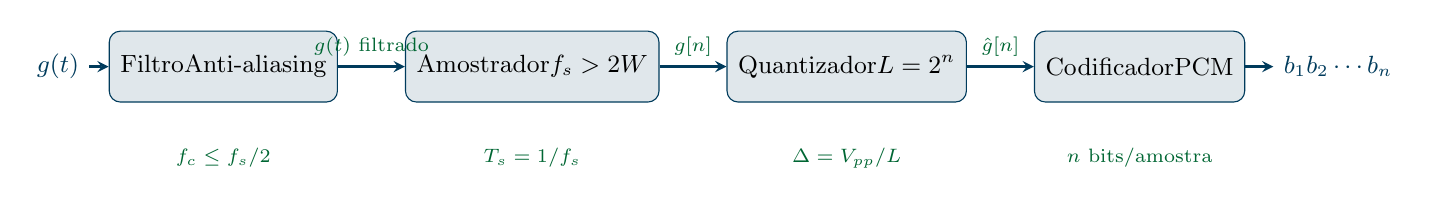
\begin{tikzpicture}[
    adcblk/.style={draw, rectangle, rounded corners=4pt,
                   minimum width=2.1cm, minimum height=0.9cm,
                   text centered, fill=unbprimary!12,
                   draw=unbprimary, font=\small, inner sep=4pt},
    arw/.style={->, thick, >=stealth, color=unbprimary},
    lbl/.style={font=\scriptsize, color=unbsecondary, text centered}
  ]
    % Blocos
    \node[adcblk]                      (aa)   {Filtro\\Anti-aliasing};
    \node[adcblk, right=0.85cm of aa]  (samp) {Amostrador\\$f_s > 2W$};
    \node[adcblk, right=0.85cm of samp](quant){Quantizador\\$L = 2^n$};
    \node[adcblk, right=0.85cm of quant](enc) {Codificador\\PCM};

    % Setas e rótulos de sinal
    \draw[arw] (-1.7,0) node[left, font=\small]{$g(t)$} -- (aa);
    \draw[arw] (aa)    -- (samp)  node[midway,above,lbl]{$g(t)$ filtrado};
    \draw[arw] (samp)  -- (quant) node[midway,above,lbl]{$g[n]$};
    \draw[arw] (quant) -- (enc)   node[midway,above,lbl]{$\hat{g}[n]$};
    \draw[arw] (enc)   -- ++(1.7,0)
                       node[right, font=\small]{$b_1 b_2\cdots b_n$};

    % Parâmetros abaixo de cada bloco
    \node[lbl, below=0.45cm of aa]   {$f_c \le f_s/2$};
    \node[lbl, below=0.45cm of samp] {$T_s = 1/f_s$};
    \node[lbl, below=0.45cm of quant]{$\Delta = V_{pp}/L$};
    \node[lbl, below=0.45cm of enc]  {$n$ bits/amostra};
  \end{tikzpicture}
  \end{center}

  \vspace{0.4cm}
  Cada etapa tem parâmetros de projeto que determinam a
  qualidade e a taxa de bits resultante.
\end{frame}

% ------------------------------------------------------------------

\begin{frame}{Codificação Binária: PCM}
  Após a quantização, cada nível $\hat{g}[n]$ recebe uma
  \textbf{palavra binária de $n$ bits} (representação PCM).

  \vspace{0.3cm}
  Com $n$ bits podemos representar $L = 2^n$ níveis:
  \[
    L = 2^n
    \quad\Longleftrightarrow\quad
    n = \log_2 L
  \]

  \vspace{0.3cm}
  \textbf{Exemplo com $n = 3$ bits ($L = 8$ níveis):}

  \vspace{0.2cm}
  \begin{center}
  \begin{tabular}{ccc}
    \hline
    Índice $k$ & Código binário & Nível $\hat{g}$\\
    \hline
    0 & \texttt{000} & $V_{\min} + 0{,}5\Delta$ \\
    1 & \texttt{001} & $V_{\min} + 1{,}5\Delta$ \\
    $\vdots$ & $\vdots$ & $\vdots$ \\
    7 & \texttt{111} & $V_{\min} + 7{,}5\Delta$ \\
    \hline
  \end{tabular}
  \end{center}
\end{frame}

% ------------------------------------------------------------------

\begin{frame}{Taxa de Bits e Largura de Banda PCM}
  A \textbf{taxa de bits} (bit rate) do canal PCM é:
  \[
    R_b = n \cdot f_s \quad \text{[bits/s]}
  \]
  onde $n$ é o número de bits por amostra e
  $f_s$ é a taxa de amostragem.

  \vspace{0.35cm}
  A largura de banda mínima necessária para transmitir o PCM
  (sem inter-símbolos) é:
  \[
    B_{\min} = \frac{R_b}{2} = \frac{n\,f_s}{2}
  \]

  \vspace{0.35cm}
  \textbf{Compromisso clássico:}
  \begin{itemize}
    \item Qualidade alta $\Rightarrow$ $n$ grande $\Rightarrow$ $R_b$ alto
          $\Rightarrow$ mais largura de banda
    \item Largura de banda limitada $\Rightarrow$ $n$ reduzido
          $\Rightarrow$ mais ruído de quantização
  \end{itemize}
\end{frame}

% ------------------------------------------------------------------

\begin{frame}{Exemplo de Projeto PCM: Telefonia Digital}
  \textbf{Parâmetros do canal de voz (ITU-T G.711):}

  \vspace{0.2cm}
  \begin{itemize}
    \item Largura de banda da voz: $W = 4\,\text{kHz}$
    \item Taxa de amostragem escolhida: $f_s = 8\,\text{kHz}$
          \quad (garante $f_s > 2W$, com margem)
    \item Resolução: $n = 8$ bits/amostra ($L = 256$ níveis)
  \end{itemize}

  \vspace{0.35cm}
  \textbf{Taxa de bits por canal:}
  \[
    R_b = n \cdot f_s = 8 \times 8\,000 = 64\,\text{kb/s}
  \]

  \textbf{SQNR máximo (senoide):}
  \[
    \SQNR_{\mathrm{dB}} \approx 1{,}76 + 6{,}02 \times 8 \approx 50\,\text{dB}
  \]

  \vspace{0.2cm}
  \textbf{Observação:} 50 dB é adequado para inteligibilidade da voz,
  mas ainda abaixo da qualidade de áudio de alta fidelidade (CD: $\sim$98 dB).
\end{frame}

% ------------------------------------------------------------------
\subsection{Companding}
% ------------------------------------------------------------------

\begin{frame}{Por Que Companding? Motivação}
  \textbf{Problema com quantização uniforme para a voz:}

  \vspace{0.2cm}
  A amplitude da voz humana \textbf{não tem distribuição uniforme} —
  amplitudes pequenas são muito mais frequentes do que amplitudes grandes.

  \vspace{0.35cm}
  Com quantização uniforme:
  \begin{itemize}
    \item Os poucos níveis disponíveis se distribuem \textbf{igualmente}
          por toda a faixa
    \item A maioria das amostras (pequena amplitude) usa apenas
          uma \alert{pequena fração} dos níveis
    \item Para sinais fracos, o SQNR cai drasticamente
  \end{itemize}

  \vspace{0.35cm}
  \textbf{Solução:} usar passos $\Delta$ \textbf{menores perto de zero}
  e maiores para amplitudes altas.\\
  Isso é a \alert{quantização não-uniforme}.

  \vspace{0.25cm}
  Na prática, implementada via \textbf{companding}:
  \textbf{comp}ression + exp\textbf{anding}.
\end{frame}

% ------------------------------------------------------------------

\begin{frame}{O Conceito de Companding}
  \textbf{Companding = Compressão + Quantização Uniforme + Expansão}

  \vspace{0.35cm}
  \begin{center}
  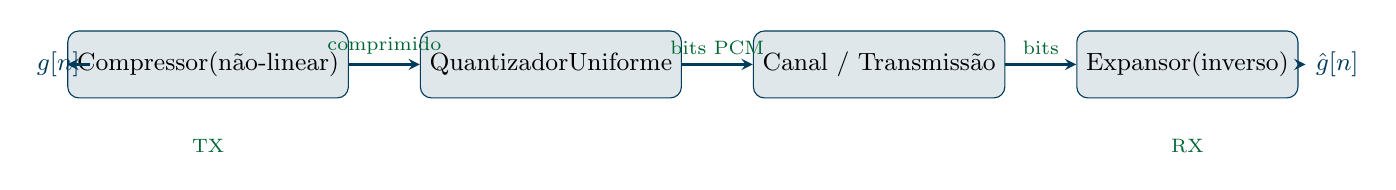
\begin{tikzpicture}[
    cmpblk/.style={draw, rectangle, rounded corners=4pt,
                   minimum width=2.0cm, minimum height=0.85cm,
                   text centered, fill=unbprimary!12,
                   draw=unbprimary, font=\small},
    arw/.style={->, thick, >=stealth, color=unbprimary},
    lbl/.style={font=\scriptsize, color=unbsecondary}
  ]
    \node[cmpblk]                       (comp)  {Compressor\\(não-linear)};
    \node[cmpblk, right=0.9cm of comp]  (quant) {Quantizador\\Uniforme};
    \node[cmpblk, right=0.9cm of quant] (chan)  {Canal / Transmissão};
    \node[cmpblk, right=0.9cm of chan]  (exp)   {Expansor\\(inverso)};

    \draw[arw] (-1.5,0) node[left, font=\small]{$g[n]$} -- (comp);
    \draw[arw] (comp)  -- (quant) node[midway,above,lbl]{comprimido};
    \draw[arw] (quant) -- (chan)  node[midway,above,lbl]{bits PCM};
    \draw[arw] (chan)  -- (exp)   node[midway,above,lbl]{bits};
    \draw[arw] (exp)   -- ++(1.5,0) node[right,font=\small]{$\hat{g}[n]$};

    \node[lbl, below=0.4cm of comp]  {TX};
    \node[lbl, below=0.4cm of exp]   {RX};
  \end{tikzpicture}
  \end{center}

  \vspace{0.3cm}
  \begin{itemize}
    \item \textbf{Compressor:} amplifica amplitudes pequenas e comprime
          amplitudes grandes antes da quantização
    \item \textbf{Expansor:} aplica a função inversa no receptor
          para restaurar as amplitudes originais
  \end{itemize}
\end{frame}

% ------------------------------------------------------------------

\begin{frame}{Lei $\mu$: Definição Matemática}
  Padrão nos EUA, Canadá e Japão (ITU-T G.711, $\mu = 255$):
  \[
    C_\mu(x) = \operatorname{sgn}(x) \,
               \frac{\ln\!\left(1 + \mu\,|x|\right)}{\ln(1 + \mu)},
               \qquad |x| \le 1
  \]

  \vspace{0.2cm}
  \textbf{Propriedades:}
  \begin{itemize}
    \item Para $\mu|x| \gg 1$ (sinal grande):
          $C_\mu(x) \approx \operatorname{sgn}(x)\,\dfrac{\ln(\mu|x|)}{\ln(1+\mu)}$
          — compressão logarítmica
    \item Para $\mu|x| \ll 1$ (sinal pequeno):
          $C_\mu(x) \approx x$ — aproximadamente linear
    \item Caso limite: $\mu \to 0$ recupera a quantização uniforme
  \end{itemize}

  \vspace{0.2cm}
  A \textbf{inversão} (expansor) é:
  \[
    C_\mu^{-1}(y) = \operatorname{sgn}(y) \,
                    \frac{(1+\mu)^{|y|} - 1}{\mu}
  \]
\end{frame}

% ------------------------------------------------------------------

\begin{frame}{Lei A: Definição Matemática}
  Padrão na Europa e em sistemas legados no Brasil
  (ITU-T G.711, $A = 87{,}6$):
  \[
    C_A(x) = \operatorname{sgn}(x)\cdot
    \begin{cases}
      \dfrac{A\,|x|}{1 + \ln A},             & 0 \le |x| < \dfrac{1}{A}\\[8pt]
      \dfrac{1 + \ln\!\left(A\,|x|\right)}{1 + \ln A},
                                              & \dfrac{1}{A} \le |x| \le 1
    \end{cases}
  \]

  \vspace{0.2cm}
  \textbf{Diferença em relação à lei $\mu$:}
  \begin{itemize}
    \item A lei A é \textbf{linear} para amplitudes muito pequenas
          ($|x| < 1/A$) e logarítmica para amplitudes maiores
    \item A lei $\mu$ é logarítmica em toda a faixa
    \item Ambas garantem SQNR quase constante
          em uma ampla faixa de níveis de sinal
  \end{itemize}
\end{frame}

% ------------------------------------------------------------------

\begin{frame}{Curvas de Compressão}
  \begin{center}
    \includegraphics[width=0.92\textwidth]{figures/cap7/companding_curves}
  \end{center}
  {\footnotesize
    A curva de compressão é côncava: a inclinação (resolução) é
    maior perto de zero e menor para grandes amplitudes.
    A linha tracejada mostra a curva linear sem compressão.
  }
\end{frame}

% ------------------------------------------------------------------

\begin{frame}{Comparação de SQNR: Uniforme vs.\ $\mu$-law}
  \begin{center}
    \includegraphics[width=0.92\textwidth]{figures/cap7/companding_sqnr_comparison}
  \end{center}
  \vspace{-0.15cm}
  {\footnotesize
    Com quantização uniforme, o SQNR cai rapidamente para sinais fracos.
    Com $\mu$-law, o SQNR permanece quase constante ao longo de uma
    ampla faixa dinâmica — essencial para a voz humana.
  }
\end{frame}

% ------------------------------------------------------------------

\begin{frame}[fragile]{Implementação em Python: $\mu$-law Companding}
\begin{lstlisting}[language=Python]
import numpy as np

def mu_law_compress(x, mu=255):
    return np.sign(x) * np.log(1 + mu*np.abs(x)) / np.log(1 + mu)

def mu_law_expand(y, mu=255):
    return np.sign(y) * (1/mu) * ((1+mu)**np.abs(y) - 1)

def quantize_uniform(x, n_bits, v_min=-1.0, v_max=1.0):
    L   = 2**n_bits
    d   = (v_max - v_min) / L
    idx = np.clip(np.floor((np.clip(x, v_min, v_max)-v_min)/d), 0, L-1)
    return v_min + (idx.astype(int) + 0.5) * d

# Pipeline de companding
g        = 0.05 * np.sin(2*np.pi*np.linspace(0,100,1_000_000))
g_comp   = mu_law_compress(g)          # compressao
g_q_comp = quantize_uniform(g_comp, 8) # quantizacao uniforme
g_rec    = mu_law_expand(g_q_comp)     # expansao
sqnr_mu  = 10*np.log10(np.mean(g**2)/np.mean((g_rec - g)**2))
print(f"SQNR mu-law: {sqnr_mu:.1f} dB")
\end{lstlisting}
\end{frame}

% ------------------------------------------------------------------
\subsection{Resumo}
% ------------------------------------------------------------------

\begin{frame}{Resumo: Conversão Analógico-Digital}
  \begin{block}{Resultado 1 — Amostragem (Nyquist-Shannon)}
    \[
      f_s > 2W
      \qquad\Longrightarrow\qquad
      G_s(f) = f_s\sum_{k=-\infty}^{\infty} G(f - k\,f_s)
    \]
  \end{block}

  \vspace{0.25cm}

  \begin{block}{Resultado 2 — Ruído de Quantização}
    \[
      P_q = \frac{\Delta^2}{12},
      \qquad
      \Delta = \frac{V_{pp}}{2^n}
    \]
  \end{block}

  \vspace{0.25cm}

  \begin{block}{Resultado 3 — SQNR (senoide em faixa cheia)}
    \[
      \SQNR_{\mathrm{dB}} \approx 1{,}76 + 6{,}02\,n \;\text{dB}
      \qquad\longleftarrow\quad 6\text{ dB por bit}
    \]
  \end{block}

  \vspace{0.2cm}
  \textbf{Companding} ($\mu$-law / A-law) mantém SQNR quase constante
  para sinais com distribuição de amplitude não-uniforme (ex.: voz).
\end{frame}



% %%%%%%%%%%%%%%%%%%%%%%%%%%%%%%%%%%%%%%%%%%%%
% SLIDE DE TRANSIÇÃO: CAPÍTULO 6
% %%%%%%%%%%%%%%%%%%%%%%%%%%%%%%%%%%%%%%%%%%%%
{
\setbeamercolor{background canvas}{bg=structure.fg}
\setbeamercolor{normal text}{fg=white}
\usebeamercolor[fg]{normal text}
\begin{frame}[plain,c]
\begin{center}
{\Huge\textbf{Capítulo 6}}\\[0.8cm]
{\LARGE Princípios de Transmissão Digital}\\[0.5cm]
{\large Codificação de Linha, Formatação de Pulso,\\
Diagrama de Olho e PAM M-ário}
\end{center}
\end{frame}
}

% ============================================
% CAPÍTULO 6: TRANSMISSÃO DIGITAL DE DADOS
% ============================================
% ============================================
% CAPÍTULO 6: PRINCÍPIOS DE TRANSMISSÃO DIGITAL
% ============================================
% Este arquivo organiza o conteúdo do Capítulo 6
% sobre Transmissão Digital de Dados em Banda Base

% ============================================
% SISTEMAS DE COMUNICAÇÃO DIGITAL
% ============================================
\section{Sistemas de Comunicação Digital}
% ============================================
% SEÇÃO 6.1: SISTEMAS DE COMUNICAÇÃO DIGITAL
% Visão geral do sistema em banda base.
% ============================================

% ------------------------------------------------------------------
\subsection{Visão Geral}
% ------------------------------------------------------------------

\begin{frame}{Onde Estamos na Cadeia?}
  \drawpipeline{linecoder,pulseshaper,channel,detector}
  \vspace{0.1cm}
  {\small Neste capítulo: os bits produzidos pelo PCM precisam ser
  transmitidos pelo canal. Estudamos como mapear bits em formas de onda,
  controlar a banda ocupada e tomar decisões no receptor.}
\end{frame}

\begin{frame}{O que é Transmissão Digital em Banda Base?}
  Na \alert{transmissão em banda base}, o sinal digital é enviado
  \textbf{diretamente} pelo canal, sem modulação por portadora.

  \vspace{0.4cm}
  \textbf{Exemplos práticos:}
  \begin{itemize}
    \item Comunicação interna em computadores (barramentos)
    \item Ethernet cabeada (10BASE-T, 100BASE-TX)
    \item Linha telefônica digital (DSL — trecho local)
    \item USB, HDMI, PCIe
  \end{itemize}

  \vspace{0.4cm}
  \textit{A ideia central: representar bits como formas de onda
  elétrica e transmiti-los por um canal com ruído e limitação de banda.}
\end{frame}

% ------------------------------------------------------------------

\begin{frame}{Cadeia de Transmissão Digital}
  \begin{center}
    \includegraphics[width=0.82\textwidth]{figures/cap6/digital_comm_system}
  \end{center}
  \vspace{-0.2cm}
  {\footnotesize
    A fonte gera símbolos $\{a_k\}$; o codificador de linha mapeia em
    níveis elétricos; o formatador de pulso gera $s(t)$; o canal adiciona
    ruído $n(t)$; o receptor filtra e decide $\hat{a}_k$.}
\end{frame}

% ------------------------------------------------------------------

\begin{frame}{Elementos do Sistema}
  \textbf{1. Fonte digital} — gera uma sequência de símbolos $\{a_k\}$,
  onde cada $a_k$ pertence a um alfabeto de $M$ níveis.

  \vspace{0.3cm}
  \textbf{2. Formatação de pulso} — o sinal transmitido é:
  \[
    s(t) = \sum_{k=-\infty}^{\infty} a_k\, p(t - kT)
  \]
  onde $p(t)$ é o \alert{pulso básico} e $T$ é o \alert{intervalo de sinalização}.

  \vspace{0.3cm}
  \textbf{3. Canal} — introduz atenuação, distorção e ruído aditivo $n(t)$:
  \[
    r(t) = s(t) * h_c(t) + n(t)
  \]

  \vspace{0.3cm}
  \textbf{4. Receptor} — filtra $r(t)$, amostra em $t = kT$ e decide
  qual símbolo $\hat{a}_k$ foi enviado.
\end{frame}

% ------------------------------------------------------------------

\begin{frame}{Taxas Fundamentais}
  Para um sistema $M$-ário com intervalo de símbolo $T$:

  \vspace{0.3cm}
  \textbf{Taxa de sinalização} (taxa de símbolos):
  \[
    R_s = \frac{1}{T} \quad \text{[símbolos/s ou \textit{baud}]}
  \]

  \vspace{0.3cm}
  \textbf{Taxa de bits:}
  \[
    R_b = R_s \cdot \log_2 M = \frac{\log_2 M}{T} \quad \text{[bits/s]}
  \]

  \vspace{0.3cm}
  \textit{Exemplo:} Um sistema 4-PAM ($M=4$) com $R_s = 1000$ baud
  transmite $R_b = 1000 \times 2 = 2000$ bits/s — o \alert{dobro}
  da taxa de um sistema binário na mesma banda.
\end{frame}


% ============================================
% CODIFICAÇÃO DE LINHA
% ============================================
\section{Codificação de Linha}
% ============================================
% SEÇÃO 6.2: CODIFICAÇÃO DE LINHA
% Principais formatos e suas propriedades.
% ============================================

% ------------------------------------------------------------------
\subsection{O que é Codificação de Linha?}
% ------------------------------------------------------------------

\begin{frame}{Onde Estamos na Cadeia?}
  \drawpipeline{linecoder}
  \vspace{0.1cm}
  {\small Nesta seção: \textbf{Codificador de Linha} — como converter
  bits em níveis de tensão, escolhendo o formato adequado para
  banda, sincronismo e componente DC.}
\end{frame}

\begin{frame}{Motivação}
  Antes de transmitir, precisamos escolher \textbf{como representar}
  cada bit (ou grupo de bits) como uma forma de onda elétrica.

  \vspace{0.3cm}
  A \alert{codificação de linha} define o mapeamento:
  \[
    \text{bit } b_k \;\longrightarrow\; \text{nível de tensão } a_k
    \;\longrightarrow\; \text{pulso } a_k\, p(t - kT_b)
  \]

  \vspace{0.3cm}
  \textbf{Critérios de escolha:}
  \begin{itemize}
    \item \textbf{Largura de banda} — quanto espectro o código ocupa?
    \item \textbf{Componente DC} — zero é desejável (acoplamento AC)
    \item \textbf{Sincronismo} — o código facilita recuperação de relógio?
    \item \textbf{Detecção de erros} — violações indicam erros?
    \item \textbf{Complexidade} — custo de implementação
  \end{itemize}
\end{frame}

% ------------------------------------------------------------------
\subsection{Códigos Clássicos}
% ------------------------------------------------------------------

\begin{frame}{Unipolar NRZ e Polar NRZ}
  \textbf{Unipolar NRZ} (\textit{Non-Return-to-Zero}):
  \[
    a_k = \begin{cases} A, & b_k = 1 \\ 0, & b_k = 0 \end{cases}
  \]
  \begin{itemize}
    \item Simples, mas tem \alert{componente DC} — ineficiente.
    \item Longas sequências de 0s → perda de sincronismo.
  \end{itemize}

  \vspace{0.4cm}
  \textbf{Polar NRZ:}
  \[
    a_k = \begin{cases} +A, & b_k = 1 \\ -A, & b_k = 0 \end{cases}
  \]
  \begin{itemize}
    \item Sem DC \textit{na média} (bits equiprováveis).
    \item Primeiro nulo do espectro em $f = R_b = 1/T_b$.
    \item Ainda tem problema de sincronismo em sequências longas.
  \end{itemize}
\end{frame}

% ------------------------------------------------------------------

\begin{frame}{Polar RZ e Manchester}
  \textbf{Polar RZ} (\textit{Return-to-Zero}):
  \[
    a_k = \begin{cases} \pm A & \text{na 1ª metade de } T_b \\
    0 & \text{na 2ª metade de } T_b \end{cases}
  \]
  \begin{itemize}
    \item Transição garantida a cada bit → melhor para sincronismo.
    \item Porém, ocupa o \alert{dobro da banda} do NRZ.
  \end{itemize}

  \vspace{0.4cm}
  \textbf{Manchester} (Bifase):
  \[
    b_k = 1 \;\Rightarrow\; +A \text{ (1ª metade)},\; -A \text{ (2ª metade)}
  \]
  \[
    b_k = 0 \;\Rightarrow\; -A \text{ (1ª metade)},\; +A \text{ (2ª metade)}
  \]
  \begin{itemize}
    \item \alert{Sem componente DC} — transição no meio de cada bit.
    \item Usado em Ethernet 10BASE-T.
    \item Largura de banda: primeiro nulo em $f = 2R_b$.
  \end{itemize}
\end{frame}

% ------------------------------------------------------------------

\begin{frame}{AMI — Inversão de Marca Alternada}
  No código \textbf{AMI} (\textit{Alternate Mark Inversion}):
  \[
    b_k = 0 \;\Rightarrow\; a_k = 0 \qquad
    b_k = 1 \;\Rightarrow\; a_k = +A \text{ ou } -A \;\text{(alternado)}
  \]

  \vspace{0.3cm}
  \textit{Cada ``1'' alterna a polaridade em relação ao ``1'' anterior.}

  \vspace{0.3cm}
  \textbf{Vantagens:}
  \begin{itemize}
    \item \alert{Componente DC = 0} por construção.
    \item Violação da regra de alternância → \textbf{detecção de erros}.
    \item PSD concentrada em frequências mais baixas.
  \end{itemize}

  \vspace{0.3cm}
  \textbf{Desvantagem:} longas sequências de ``0'' causam perda de
  sincronismo (o sinal fica em zero). \\
  \textit{Solução: usar \textbf{scrambling} (embaralhamento) ou
  códigos derivados como HDB3 e B8ZS.}
\end{frame}

% ------------------------------------------------------------------
\subsection{Formas de Onda e Espectros}
% ------------------------------------------------------------------

\begin{frame}{Comparação Visual das Codificações}
  \begin{center}
    \includegraphics[width=0.78\textwidth]{figures/cap6/line_coding_waveforms}
  \end{center}
  \vspace{-0.2cm}
  {\footnotesize
    Sequência de bits $[1,0,1,1,0,0,1,0]$ codificada em seis formatos diferentes.
    Note as transições e os níveis de tensão de cada código.}
\end{frame}

% ------------------------------------------------------------------

\begin{frame}{Densidade Espectral de Potência}
  \begin{center}
    \includegraphics[width=0.82\textwidth]{figures/cap6/line_coding_psd}
  \end{center}
  \vspace{-0.2cm}
  {\footnotesize
    A PSD do \textbf{Polar NRZ} tem primeiro nulo em $f = R_b$;
    \textbf{Manchester} tem nulo em $f = 2R_b$ (dobro da banda);
    \textbf{AMI} vai a zero em $f = 0$ (sem DC) e em $f = R_b$.}
\end{frame}

% ------------------------------------------------------------------
\subsection{Resumo Comparativo}
% ------------------------------------------------------------------

\begin{frame}{Tabela Comparativa dos Códigos de Linha}
  \vspace{0.2cm}
  \begin{center}
  \renewcommand{\arraystretch}{1.3}
  \footnotesize
  \begin{tabular}{l c c c c}
    \hline
    \textbf{Código} & \textbf{BW mín.} & \textbf{DC = 0?} &
    \textbf{Sincronismo} & \textbf{Detecção} \\
    \hline
    Unipolar NRZ   & $R_b$    & Não  & Ruim   & Não \\
    Polar NRZ       & $R_b$    & Sim* & Ruim   & Não \\
    Polar RZ        & $2R_b$   & Sim* & Bom    & Não \\
    Manchester      & $2R_b$   & Sim  & Ótimo  & Não \\
    AMI (NRZ)       & $R_b$    & Sim  & Médio  & Sim \\
    Bipolar RZ      & $R_b$    & Sim  & Bom    & Sim \\
    \hline
  \end{tabular}
  \end{center}
  \vspace{0.2cm}
  {\footnotesize *Na média, para bits equiprováveis.
  \textbf{BW mín.} = largura de banda do primeiro lóbulo espectral.}

  \vspace{0.2cm}
  \textit{Não existe código perfeito — a escolha depende dos requisitos
  do sistema (banda disponível, necessidade de sincronismo, etc.).}
\end{frame}


% ============================================
% FORMATAÇÃO DE PULSO
% ============================================
\section{Formatação de Pulso e ISI}
% ============================================
% SEÇÃO 6.3: FORMATAÇÃO DE PULSO E ISI
% Critério de Nyquist, pulso cosseno levantado.
% ============================================

% ------------------------------------------------------------------
\subsection{Interferência Intersimbólica (ISI)}
% ------------------------------------------------------------------

\begin{frame}{Onde Estamos na Cadeia?}
  \drawpipeline{pulseshaper}
  \vspace{0.1cm}
  {\small Nesta seção: \textbf{Formatador de Pulso} — a escolha do pulso
  $p(t)$ determina a banda ocupada e a sensibilidade à ISI.
  O critério de Nyquist e o cosseno levantado são as ferramentas centrais.}
\end{frame}

\begin{frame}{O Problema da ISI}
  Considere o sinal transmitido:
  \[
    s(t) = \sum_{k} a_k\, p(t - kT)
  \]

  No receptor, amostramos $r(t)$ nos instantes $t = nT$:
  \[
    r(nT) = \underbrace{a_n\, p(0)}_{\text{símbolo desejado}}
    + \underbrace{\sum_{k \neq n} a_k\, p(nT - kT)}_{\text{ISI}}
    + n(nT)
  \]

  \vspace{0.3cm}
  Se $p(t)$ for ``largo demais'', as \alert{caudas} de pulsos vizinhos
  contaminam o instante de amostragem → \textbf{Interferência Intersimbólica (ISI)}.

  \vspace{0.3cm}
  \textit{A ISI é tão prejudicial quanto o ruído — e pode ser eliminada
  com a escolha adequada de $p(t)$.}
\end{frame}

% ------------------------------------------------------------------

\begin{frame}{Visualização da ISI}
  \begin{center}
    \includegraphics[width=0.78\textwidth]{figures/cap6/pulse_shaping_isi}
  \end{center}
  \vspace{-0.2cm}
  {\footnotesize
    (a) Pulsos sinc ideais têm zeros em $t = nT$ ($n \neq 0$) → sem ISI.
    (b) Pulsos mais ``gordos'' geram sobreposição → ISI nos instantes de decisão.}
\end{frame}

% ------------------------------------------------------------------
\subsection{Critério de Nyquist para Zero ISI}
% ------------------------------------------------------------------

\begin{frame}{Condição para ISI Nula}
  Para eliminar a ISI, precisamos que $p(t)$ satisfaça:
  \[
    p(nT) = \begin{cases} 1, & n = 0 \\ 0, & n \neq 0 \end{cases}
  \]

  \vspace{0.2cm}
  Isso equivale, no domínio da frequência, ao \alert{Critério de Nyquist}:
  \[
    \sum_{k=-\infty}^{\infty} P\!\left(f - \frac{k}{T}\right) = T
    \quad \forall\, f
  \]

  \vspace{0.3cm}
  \textit{Interpretação:} quando ``dobramos'' (somamos réplicas de) $P(f)$
  com espaçamento $1/T$, o resultado deve ser \textbf{constante}.

  \vspace{0.2cm}
  O pulso mais simples que satisfaz isso é o $\sinc$:
  \[
    p(t) = \sinc\!\left(\frac{t}{T}\right) \quad \Longleftrightarrow \quad
    P(f) = T\,\rect(fT)
  \]
  Banda mínima: $W = \dfrac{1}{2T}$ (filtro retangular ideal).
\end{frame}

% ------------------------------------------------------------------

\begin{frame}{Problema do Pulso Sinc Puro}
  O pulso $\sinc(t/T)$ é \textbf{matematicamente perfeito}, mas na prática:

  \vspace{0.3cm}
  \begin{itemize}
    \item \textbf{Decaimento lento} — caudas decaem como $1/t$ apenas.
    \item Pequeno \alert{erro de temporização} $\epsilon$ causa ISI severa
          (a série $\sum 1/n$ diverge!).
    \item \textbf{Não é realizável} — resposta ao impulso infinita e não causal.
  \end{itemize}

  \vspace{0.4cm}
  \textit{Solução prática:} usar um pulso com \textbf{banda extra}
  (roll-off) que ainda satisfaz o critério de Nyquist, mas cujas
  caudas decaem mais rápido → \alert{Cosseno Levantado}.
\end{frame}

% ------------------------------------------------------------------
\subsection{Pulso Cosseno Levantado}
% ------------------------------------------------------------------

\begin{frame}{Definição — Domínio da Frequência}
  O espectro do \alert{cosseno levantado} com fator de
  \textit{roll-off} $\alpha \in [0, 1]$:
  \[
    P(f) = \begin{cases}
      T, & |f| \le \dfrac{1-\alpha}{2T} \\[8pt]
      \dfrac{T}{2}\left[1 + \cos\!\left(
        \dfrac{\pi T}{\alpha}\left(|f| - \dfrac{1-\alpha}{2T}\right)
      \right)\right], & \dfrac{1-\alpha}{2T} < |f| \le \dfrac{1+\alpha}{2T} \\[8pt]
      0, & |f| > \dfrac{1+\alpha}{2T}
    \end{cases}
  \]

  \vspace{0.2cm}
  A \textbf{largura de banda} ocupada é:
  \[
    W = \frac{1+\alpha}{2T}
  \]

  \vspace{0.1cm}
  {\footnotesize
  $\alpha = 0$: banda mínima ($W = 1/2T$), mas caudas lentas (sinc puro). \\
  $\alpha = 1$: dobro da banda ($W = 1/T$), mas caudas decaem como $1/t^3$ — muito mais robusto.}
\end{frame}

% ------------------------------------------------------------------

\begin{frame}{Definição — Domínio do Tempo}
  No tempo, o pulso cosseno levantado é:
  \[
    p(t) = \sinc\!\left(\frac{t}{T}\right) \cdot
    \frac{\cos\!\left(\dfrac{\pi \alpha\, t}{T}\right)}
    {1 - \left(\dfrac{2\alpha\, t}{T}\right)^{\!2}}
  \]

  \vspace{0.3cm}
  \textbf{Observação importante:}
  \begin{itemize}
    \item O fator $\sinc(t/T)$ garante zeros em $t = nT$ → critério de Nyquist.
    \item O fator cosseno/denominador acelera o decaimento das caudas.
    \item Para $\alpha > 0$, as caudas decaem como $\sim 1/|t|^3$.
  \end{itemize}

  \vspace{0.2cm}
  \textit{Quanto maior $\alpha$, mais robusto ao erro de temporização,
  porém maior a banda ocupada.}
\end{frame}

% ------------------------------------------------------------------
\subsection{Visualização}
% ------------------------------------------------------------------

\begin{frame}{Cosseno Levantado: Tempo e Frequência}
  \begin{columns}[T]
    \column{0.49\textwidth}
    \textbf{Domínio do tempo}
    \begin{center}
      \includegraphics[width=\textwidth]{figures/cap6/raised_cosine_time}
    \end{center}
    {\scriptsize
      Todos os pulsos passam por zero em $t = nT$.
      Com $\alpha = 1$, as caudas decaem como $1/|t|^3$.}

    \column{0.49\textwidth}
    \textbf{Domínio da frequência}
    \begin{center}
      \includegraphics[width=\textwidth]{figures/cap6/raised_cosine_freq}
    \end{center}
    {\scriptsize
      $\alpha = 0$: filtro retangular (banda mínima $1/2T$).
      $\alpha = 1$: transição suave, banda dobrada $1/T$.}
  \end{columns}
\end{frame}

% ------------------------------------------------------------------

\begin{frame}{Comparação: Retangular vs.\ Sinc vs.\ Cosseno Levantado}
  \begin{center}
    \includegraphics[width=0.88\textwidth]{figures/cap6/pulse_shaping_comparison}
  \end{center}
  \vspace{-0.2cm}
  {\footnotesize
    O sinal total resulta da soma de pulsos deslocados. Em (a), as
    descontinuidades causam banda infinita. Em (b) e (c), a suavização
    limita o espectro, mas apenas (b) e (c) eliminam ISI nos instantes $nT$.}
\end{frame}

% ------------------------------------------------------------------
\subsection{Eficiência Espectral}
% ------------------------------------------------------------------

\begin{frame}{Relação Banda--Taxa}
  Com pulso cosseno levantado de roll-off $\alpha$, a banda necessária é:
  \[
    W = \frac{1 + \alpha}{2T} = \frac{(1+\alpha)\, R_s}{2}
  \]

  \vspace{0.2cm}
  A \textbf{eficiência espectral} (para sistema binário) é:
  \[
    \eta = \frac{R_b}{W} = \frac{2}{1 + \alpha} \quad
    \text{[bits/s/Hz]}
  \]

  \vspace{0.3cm}
  \begin{center}
  \renewcommand{\arraystretch}{1.2}
  \footnotesize
  \begin{tabular}{c c c}
    \hline
    $\alpha$ & Banda $W$ & Eficiência $\eta$ \\
    \hline
    0    & $R_b/2$  & 2 bits/s/Hz \\
    0.5  & $0{,}75\, R_b$ & 1{,}33 bits/s/Hz \\
    1.0  & $R_b$    & 1 bit/s/Hz \\
    \hline
  \end{tabular}
  \end{center}

  \vspace{0.2cm}
  \textit{Na prática, $\alpha$ entre 0,2 e 0,5 oferece bom
  compromisso entre banda e robustez.}
\end{frame}


% ============================================
% DIAGRAMA DE OLHO
% ============================================
\section{Diagrama de Olho}
% ============================================
% SEÇÃO 6.4: DIAGRAMA DE OLHO
% Ferramenta de diagnóstico visual.
% ============================================

% ------------------------------------------------------------------
\subsection{Conceito}
% ------------------------------------------------------------------

\begin{frame}{Onde Estamos na Cadeia?}
  \drawpipeline{channel,detector}
  \vspace{0.1cm}
  {\small Nesta seção: \textbf{Canal} e \textbf{Detector} — o diagrama de
  olho é a ferramenta visual que revela o efeito do canal (ruído, ISI,
  jitter) sobre a qualidade do sinal antes da decisão.}
\end{frame}

\begin{frame}{O que é o Diagrama de Olho?}
  O \alert{diagrama de olho} (ou \textit{eye diagram}) é uma técnica
  de visualização obtida ao \textbf{sobrepor} segmentos consecutivos
  do sinal recebido, cada um com duração de 1 ou 2 intervalos de símbolo.

  \vspace{0.3cm}
  \textbf{Como construir:}
  \begin{enumerate}
    \item Receba o sinal $r(t)$ após a filtragem.
    \item Corte em trechos de duração $2T$.
    \item Sobreponha todos os trechos no mesmo gráfico.
  \end{enumerate}

  \vspace{0.3cm}
  \textit{O padrão resultante lembra um ``olho'' — e quanto mais
  \textbf{aberto} o olho, melhor a qualidade do sinal.}

  \vspace{0.3cm}
  Na prática, basta conectar o sinal a um osciloscópio com disparo
  (\textit{trigger}) sincronizado à taxa de símbolo.
\end{frame}

% ------------------------------------------------------------------
\subsection{Interpretação}
% ------------------------------------------------------------------

\begin{frame}{Leitura do Diagrama de Olho}
  O diagrama de olho revela, \textbf{de uma só vez}, diversas
  informações sobre a qualidade do enlace:

  \vspace{0.3cm}
  \begin{itemize}
    \item \textbf{Abertura vertical} → margem de ruído disponível.
    \begin{itemize}
      \item Quanto maior, mais ruído o sistema tolera.
    \end{itemize}

    \vspace{0.2cm}
    \item \textbf{Abertura horizontal} → margem de temporização (\textit{timing margin}).
    \begin{itemize}
      \item Quanto mais larga, menos sensível a \textit{jitter}.
    \end{itemize}

    \vspace{0.2cm}
    \item \textbf{Espessura das trilhas} → quantidade de ISI e ruído.
    \begin{itemize}
      \item Trilhas finas = pouco ISI; trilhas grossas = ISI severa.
    \end{itemize}

    \vspace{0.2cm}
    \item \textbf{Cruzamentos} (\textit{zero crossings}) → variações de temporização (\textit{jitter}).
  \end{itemize}
\end{frame}

% ------------------------------------------------------------------

\begin{frame}{Parâmetros do Diagrama de Olho}
  \begin{center}
    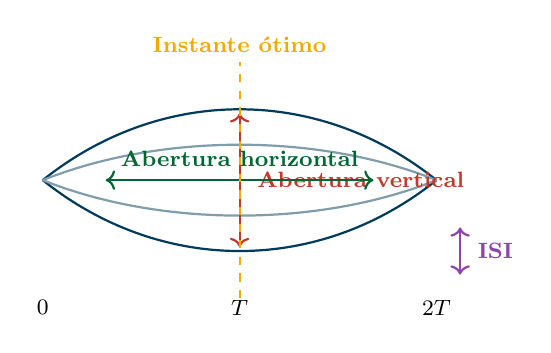
\begin{tikzpicture}[scale=1.0]
      % "Eye" shape
      \draw[thick, UNB_BLUE] (0,0) .. controls (1.5,1.2) and (3.5,1.2) .. (5,0);
      \draw[thick, UNB_BLUE] (0,0) .. controls (1.5,-1.2) and (3.5,-1.2) .. (5,0);
      \draw[thick, UNB_BLUE!50] (0,0) .. controls (1.5,0.6) and (3.5,0.6) .. (5,0);
      \draw[thick, UNB_BLUE!50] (0,0) .. controls (1.5,-0.6) and (3.5,-0.6) .. (5,0);

      % Vertical opening
      \draw[<->, thick, RED] (2.5, -0.85) -- (2.5, 0.85);
      \node[right, RED, font=\footnotesize\bfseries] at (2.6, 0) {Abertura vertical};

      % Horizontal opening
      \draw[<->, thick, UNB_GREEN] (0.8, 0) -- (4.2, 0);
      \node[above, UNB_GREEN, font=\footnotesize\bfseries] at (2.5, 0.05) {Abertura horizontal};

      % Optimal sampling
      \draw[dashed, thick, UNB_GOLD] (2.5, -1.5) -- (2.5, 1.5);
      \node[above, UNB_GOLD, font=\footnotesize\bfseries] at (2.5, 1.5) {Instante ótimo};

      % Labels
      \node[below, font=\footnotesize] at (0, -1.4) {$0$};
      \node[below, font=\footnotesize] at (2.5, -1.4) {$T$};
      \node[below, font=\footnotesize] at (5, -1.4) {$2T$};

      % ISI annotation
      \draw[<->, thick, PURPLE] (5.3, -1.2) -- (5.3, -0.6);
      \node[right, PURPLE, font=\footnotesize\bfseries] at (5.4, -0.9) {ISI};
    \end{tikzpicture}
  \end{center}

  \vspace{0.2cm}
  {\footnotesize
    A abertura vertical indica a \textbf{margem de ruído};
    a horizontal, a \textbf{margem de temporização}.
    O instante ótimo de amostragem é no centro do olho.}
\end{frame}

% ------------------------------------------------------------------
\subsection{Exemplos Práticos}
% ------------------------------------------------------------------

\begin{frame}{Diagrama de Olho: Canal e Efeito do Roll-off}
  \begin{columns}[T]
    \column{0.49\textwidth}
    \textbf{Canal limpo vs.\ ruidoso}
    \begin{center}
      \includegraphics[width=\textwidth]{figures/cap6/eye_diagram_clean}
    \end{center}
    {\scriptsize
      (a) Olho bem aberto — margem confortável.
      (b) Com ruído, o olho ``fecha''.}

    \column{0.49\textwidth}
    \textbf{Efeito do roll-off $\alpha$}
    \begin{center}
      \includegraphics[width=\textwidth]{figures/cap6/eye_diagram_rolloff}
    \end{center}
    {\scriptsize
      $\alpha = 0$: olho estreito (sensível a jitter).
      $\alpha = 1$: olho mais largo e robusto.}
  \end{columns}
\end{frame}


% ============================================
% PAM M-ÁRIO
% ============================================
\section{PAM: Sinalização M-ária}
% ============================================
% SEÇÃO 6.5: PAM — SINALIZAÇÃO M-ÁRIA
% Extensão para múltiplos níveis.
% ============================================

% ------------------------------------------------------------------
\subsection{Motivação para M-PAM}
% ------------------------------------------------------------------

\begin{frame}{Onde Estamos na Cadeia?}
  \drawpipeline{pulseshaper,detector}
  \vspace{0.1cm}
  {\small Nesta seção: \textbf{$M$-PAM} — ampliamos o alfabeto de
  símbolos para $M$ níveis, aumentando a eficiência espectral ao
  custo de maior sensibilidade ao ruído.}
\end{frame}

\begin{frame}{Por que Usar Mais de 2 Níveis?}
  No sistema binário (2-PAM), cada símbolo carrega \textbf{1 bit}.

  \vspace{0.3cm}
  Se usarmos $M$ níveis de amplitude (\alert{$M$-PAM}), cada símbolo
  carrega $\log_2 M$ bits:
  \[
    R_b = R_s \cdot \log_2 M
  \]

  \vspace{0.2cm}
  Para uma mesma banda $W$, podemos \textbf{aumentar a taxa de bits}
  sem aumentar a taxa de símbolos $R_s$ — ou, equivalentemente,
  manter $R_b$ e \alert{reduzir pela metade} a banda a cada
  duplicação de $M$.

  \vspace{0.3cm}
  \textit{Exemplo prático:} Ethernet 2.5GBASE-T e 5GBASE-T usam
  \textbf{PAM-4} e \textbf{PAM-16} para atingir altas taxas em
  cabos de par trançado.
\end{frame}

% ------------------------------------------------------------------
\subsection{Definição do Sinal M-PAM}
% ------------------------------------------------------------------

\begin{frame}{Sinal $M$-PAM}
  O sinal transmitido é:
  \[
    s(t) = \sum_{k} a_k\, p(t - kT)
  \]
  onde agora $a_k \in \{-(M-1),\; -(M-3),\; \ldots,\; +(M-3),\; +(M-1)\}$.

  \vspace{0.3cm}
  Os $M$ níveis são \textbf{igualmente espaçados} com distância $2d$:
  \[
    a_k \in \{(2m - 1 - M)\, d \;:\; m = 1, 2, \ldots, M\}
  \]

  \vspace{0.3cm}
  \textit{Exemplo para 4-PAM} ($M = 4$, $d = 1$):
  \[
    a_k \in \{-3,\; -1,\; +1,\; +3\}
  \]
  Cada símbolo representa $\log_2 4 = 2$ bits:
  $00 \to -3$, $01 \to -1$, $10 \to +1$, $11 \to +3$.
\end{frame}

% ------------------------------------------------------------------
\subsection{Constelação e Formas de Onda}
% ------------------------------------------------------------------

\begin{frame}{Constelações PAM}
  \begin{center}
    \includegraphics[width=0.78\textwidth]{figures/cap6/pam_constellation}
  \end{center}
  \vspace{-0.2cm}
  {\footnotesize
    A ``constelação'' de um sinal $M$-PAM é um conjunto de pontos
    sobre uma linha real. As linhas tracejadas indicam os limiares de
    decisão. Com mais níveis, a distância entre vizinhos diminui.}
\end{frame}

% ------------------------------------------------------------------

\begin{frame}{Comparação de Formas de Onda: 2-PAM vs.\ 4-PAM}
  \begin{center}
    \includegraphics[width=0.78\textwidth]{figures/cap6/pam_waveforms}
  \end{center}
  \vspace{-0.2cm}
  {\footnotesize
    Em (a), cada bit gera um símbolo — taxa de símbolo igual à de bits.
    Em (b), dois bits são agrupados em um símbolo 4-PAM — a taxa de
    símbolo cai pela metade, economizando banda.}
\end{frame}

% ------------------------------------------------------------------
\subsection{Probabilidade de Erro}
% ------------------------------------------------------------------

\begin{frame}{Decisão e Probabilidade de Erro}
  No receptor, o sinal amostrado é comparado com \textbf{limiares}:
  \[
    \hat{a}_k = \arg\min_{a_m} |r(kT) - a_m|
  \]

  \vspace{0.3cm}
  Para $M$-PAM com ruído gaussiano $\sigma^2$ e distância $2d$:

  \vspace{0.2cm}
  A probabilidade de erro de \textbf{símbolo} é:
  \[
    P_s = 2\left(1 - \frac{1}{M}\right) Q\!\left(\frac{d}{\sigma}\right)
  \]

  \vspace{0.2cm}
  onde $Q(x) = \frac{1}{\sqrt{2\pi}} \int_x^{\infty} e^{-u^2/2}\, du$.

  \vspace{0.3cm}
  \textit{Observação:} quanto maior $M$, menor a distância $d$
  (para mesma potência média), e portanto \alert{maior a taxa de erro}.
  Há um compromisso entre eficiência espectral e desempenho.
\end{frame}

% ------------------------------------------------------------------

\begin{frame}{Energia Média e SNR}
  A \textbf{energia média por símbolo} do $M$-PAM é:
  \[
    E_s = \frac{(M^2 - 1)\, d^2}{3}
  \]

  Substituindo $d = \sqrt{3 E_s / (M^2 - 1)}$ na expressão de $P_s$:
  \[
    P_s = 2\left(1 - \frac{1}{M}\right)
    Q\!\left(\sqrt{\frac{3\, E_s}{(M^2 - 1)\,\sigma^2}}\right)
  \]

  \vspace{0.3cm}
  Em termos da \textbf{energia por bit} $E_b = E_s / \log_2 M$:
  \[
    P_s = 2\left(1 - \frac{1}{M}\right)
    Q\!\left(\sqrt{\frac{3\, \log_2 M}{M^2 - 1} \cdot
    \frac{2 E_b}{N_0}}\right)
  \]

  \vspace{0.2cm}
  \textit{Aumentar $M$ exige maior $E_b/N_0$ para manter a mesma
  $P_s$ — é o ``custo'' da eficiência espectral.}
\end{frame}

% ------------------------------------------------------------------
\subsection{Diagrama de Olho M-PAM}
% ------------------------------------------------------------------

\begin{frame}{Diagrama de Olho para 4-PAM}
  \begin{center}
    \includegraphics[width=0.78\textwidth]{figures/cap6/eye_diagram_4pam}
  \end{center}
  \vspace{-0.2cm}
  {\footnotesize
    Com 4 níveis, aparecem 3 ``olhos'' empilhados. As linhas tracejadas
    amarelas indicam os limiares de decisão. O olho central é menor que
    no caso binário — \alert{maior sensibilidade ao ruído}.}
\end{frame}

% ------------------------------------------------------------------
\subsection{Resumo do Capítulo}
% ------------------------------------------------------------------

\begin{frame}{Resumo — Transmissão Digital em Banda Base}
  \textbf{Codificação de Linha:} define como bits viram formas de onda.
  Códigos como Polar NRZ, Manchester e AMI têm diferentes compromissos
  em banda, DC e sincronismo.

  \vspace{0.3cm}
  \textbf{Formatação de Pulso:} o pulso $p(t)$ deve satisfazer o
  critério de Nyquist para eliminar ISI. O cosseno levantado com
  roll-off $\alpha$ é a escolha padrão:
  \[
    W = \frac{(1+\alpha)\, R_s}{2}
  \]

  \vspace{0.3cm}
  \textbf{Diagrama de Olho:} ferramenta visual que revela margem de
  ruído, margem de temporização e quantidade de ISI.

  \vspace{0.3cm}
  \textbf{$M$-PAM:} usando $M$ níveis, a eficiência espectral aumenta
  ($\log_2 M$ bits/símbolo), mas a sensibilidade ao ruído cresce.
\end{frame}



% ============================================
% AGRADECIMENTOS
% ============================================
\begin{frame}{Agradecimentos}
\begin{center}
\Large Obrigado pela atenção!

\vspace{1cm}

\normalsize
\textbf{Contato:}\\
\autorEmail

\vspace{0.5cm}

\textbf{\laboratorioFinal}\\
\universidadeFinal

\vspace{0.5cm}

\textbf{Dúvidas?}
\end{center}
\end{frame}

% ============================================
% REFERÊNCIAS
% ============================================
\begin{frame}[allowframebreaks]{Referências}
\nocite{*}
\bibliographystyle{ieeetr}
\bibliography{references}
\end{frame}

\end{document}
